\chapter{Einführung von Tailwindcss}
\label{cha:Tailwindcss}
Tailwindcss ist ein CSS Framework, dass auf eine \textit{Utlity-First} Methodik basiert. Dabei werden CSS-Klassen überwiegend als atomare Attribute definiert, die abschließend bei Bedarf in Komponenten-Klassen abstrahiert werden können.

\section{Allgemeine Vorteile}
\begin{quotation}
	\emph{``We’ve had great success with going utility-first in the Algolia documentation, reducing our CSS from over 125 KB (and continuously growing) to less than 50 KB (9 KB GZipped, 7 KB with Brotli compression), \textbf{which represents a 60\% size decrease!} From a user perspective, this is a guarantee of lightning-fast loading styles with extremely low overhead.''}
	\citep{AlgoliaTailwindBlog}
\end{quotation}
Die Vorteile von Tailwindcss gegenüber anderer CSS-Frameworks sind vielseitig. Einige der von \cite{AlgoliaTailwindBlog} hervorgehobenen Eigenschaften sind insbesondere:
\begin{itemize}
  \item \textbf{Anpassbarkeit und Nachvollziehbarkeit}: Utility Klassen werden in einer JavaScript-Datei definiert und sind somit zentral einsehbar, was einfacher und schneller zu warten ist und eine gute Anpassbarkeit an individuelle Design-Systeme ermöglicht. Die Dokumentation von Tailwindcss ist außerdem leicht verständlich für Lernende.
  \item \textbf{Kontrollierbare Dateigröße}: Durch einmalig definierte Utility Klassen wächst der CSS Code nicht mehr an. Styles müsssen nicht mehr durch Spezifitäten überschrieben werden, was bessere Performance bewirkt.
  \item \textbf{Automatisierte \textit{CSS-Spülung}} (engl. purge): Da Tailwindcss initial zunächst ungenutzte viele Utility-Klassen basierend auf einer Konfiguration erstellt (Initial Größe beträgt meist unkomprimiert c.a. 2300 kB\footnote{vgl. \url{https://tailwindcss.com/docs/controlling-file-size}}) wurde das Framework mit dem Framework PurgeCSS für die Generierung von Production-Code erstellt. PurgeCSS vergleicht die gesamte Codebasis mit allen CSS-Klassen und entfernt CSS-Klassen die nicht genutzt wurden. Dadurch wird die CSS-Dateigröße meistens auf c.a. 10kB (komprimiert) reduziert \citep{TailwindcssDocsFileControll}.
  \item \textbf{Komprimierungsfreundlichkeit}: Durch Tailwindcss erfolgt die eigentliche Produktgestaltung meist direkt im Markup Code unter redundanter Verwendung von Utility-Klassennamen. Komprimierungsalgorithmen sind so gestaltet das gleiche Strings komprimiert werden, wodurch der Markup-Code durch Utlity-Klassen unwesentlich größer wird.
\end{itemize}

\section{Chanceneinschätzung für My.PORTAL}
\label{sec:Chanceneinschtzung}
Durch die Einführung von Tailwindcss erwartet die AVACO GmbH die folgenden Probleme (vgl. Kapitel \ref{cha:Herausforderungen im Frontend}) zu lösen oder zu verbessern:

\begin{itemize}
  \item \textbf{Redundante CSS Definitionen}: Scoped-CSS wird durch Tailwindcss auf ein Minimum reduziert. Redudante CSS Defintionen sollten (nahezu) vollständig entfernt werden können.
  \item \textbf{Ungenutzte CSS Klassen}: Neben Tailwinds Utlity-Klassen wird es nur in Ausnahmen andere Klassen geben. Die Chance, dass ungenutze CSS Klassen geschrieben werden wird deutlich reduziert. Ungenutze Tailwind-Klassen werden automatisch von PurgeCSS entfernt.
  \item \textbf{Post-Modularisierung von Komponenten}: Da die Styledefinitionen sich im Markup als CSS Klassen befinden sollte ein Verschieben von Code Abschnitten nur noch eine Analyse des Markups und der Script-Logik erfordern.
  \item \textbf{Tailwindkonfiguration statt Portalkonfiguration in portal-storybook} (vgl Abschnitt \ref{sec:portalConfigDep}): Es wird keine Portal-Konfiguration für die Bibliothek benötigt. Stattdessen enthält die Bibliothek eine eigene \textit{tailwind.conf.js} die sich nach der Tailwindcss Dokumentation ausrichtet. Andere Projekte nehmen diese Konfiguration dann als Basis und können sie entsprechend eigener Anforderungen zielgerichtet anpassen. (vgl. \ref{sec:ProjectCustomisation})
  \item \textbf{Property Hell}: Tailwindcss löst Vue-Properties ab die bisher dynamisch Klassen mit höherer Spezifität zur umgestaltung einer Komponentenerscheinung angelegt wurden. Stattdessen sollen Erscheinungsanpassungen mit Utility-Klassen in \textit{class}-Attributen erfolgen. Die Property Hell wird in Kapitel \ref{sec:propertyHellSolution} näher betrachtet.
\end{itemize}

Diese Einführung ist jedoch auch mit Risiken verbunden:
\begin{itemize}
  \item \textbf{Wenig allg. Langzeiterfahrung mit Tailwindcss}: Unbekannte Probleme können in der Tailwindcss-Community oder spezifisch bei der AVACO GmbH auftreten. Jedoch fällt in der Entwickler-Community  aktuell Tailwindcss verglichen mit anderen populären Frameworks (bspw. Bootstrap) auf den höchsten Zufriedenheitsgrad \citep{StateCSS2019_Frameworks}.
  \item \textbf{Technologie Konflikte}: Besonders in der Übergangsphase werden alte Technologien (z.B. SASS und Bootstrap) zusammen mit Tailwindcss und PostCSS (inkl. PurgeCSS) im Projektcode koexistieren. Die Folgen dessen können sich im Hinblick auf Bugs, Performance und Code-Komplexität stärker oder schwächer auswirken.
  \item \textbf{Bevorstehendes Upgrade auf Node 12}: Derzeit wird das Frontend auf der Node Version 11 aufgesetzt. Mit dem nächsten großen Release wird Tailwindcss Version 2 nur noch Node ab den Versionen 12 unterstützen. Da jedoch die Gebundenheit von My.PORTAL zu Version 11 derzeit primär von SASS abhängt und SASS langfristig durch Tailwindcss und PostCSS ersetzt werden wird, ist dies kein dauerhafter Risikozustand.
\end{itemize}

\section{Entwicklung}
Das Setup erfolgte gemäß der offiziellen Dokumentation\footnote{vgl. \url{https://tailwindcss.com/docs/installation}} von Tailwindcss. Damit diese Komponenten sich in anderen Projekten richtig verhalten, muss Tailwindcss auf Basis der tailwind.config.js in diesen verfügbar sein und die tailwind.css Datei aus der Bibliothek importiert werden. (vgl. Abschnitt \ref{sec:ProjectCustomisation})


\subsection{Plugins}
Die Tailwind Standardkonfiguration soll durch Plugins und Wertüberschreibung an Design-Systeme anpassbar sein. Aktuell gibt es drei Plugins:

\begin{itemize}
  \item \textbf{Color-Plugin}: Führt Corporate Identiy Farben als Utlity-Klassen ein. Es kann eine Primary Color gesetzt werden aus welcher automatisch eine passende Farbpalette für Status-Farben (Success, Error, ...) erzeugt wird. Als Basis wurde das Paket \textit{chroma-js} gewählt welches die Farbpaletten im LAB-Farbraum mischt\footnote{chroma-js LAB: \url{https://gka.github.io/chroma.js/\#chroma-lab}}. Da dieses Plugin die Konfiguration mit weiteren Object-Keys erweitert, wird es in der Konfigurationsdatei nicht als Plugin registriert sondern wird dem Konfigurationsobjekt per Spread-Syntax angehangen.
  \item \textbf{Container-Plugin}: Führt responsive Margin/Padding Größen für Container ein. Die Utility-Klasse \textit{.px-c} setzt das Padding eines Layout-Containers. Dies bietet eine größere Flexibilität beim entwickeln von Markup unter Einhaltung von Linienführungen in dem GUI.
  \item \textbf{Box-Plugin}: Definiert das Aussehen von GUI-Boxen (z.B. Karten) indem es Box-Utilitly-Klassen und eine Komponenten-Klasse (\textit{.box}) einführt.
\end{itemize}

\subsection{Anpassungsmethode in Projekten}
\label{sec:ProjectCustomisation}

Damit die Komponenten sich in die diversen Erscheinungen unterschiedlicher Portal Instanzen einpassen können, wurde eine Tailwind Setup-Methode angefertigt. Diese gibt das der Komponentenbibiliothek zugrundeliegende Tailwind-Konfigurationsobjekt zurück und bietet durch definierte Parameter die Möglichkeit das Erscheinungsbild (derzeit die Farbpalette) zu verändern. Eine tiefere Anpassung ist durch normale Tailwind Konfiguration möglich, indem Werte der Bibliothekskonfiguration verändert, entfernt oder erweitert werden. Die folgenden Codebeispiele sind referenzieren das Repository \textit{tailwindstories} (vgl. Vorbemerkung der Arbeit).

\lstinputlisting[caption={tailwind.config.js in einem Vue-Cli 3 Projekt}, label={tailwind.config.js}]{code/005-000_tailwindcss/tailwind.config.js}

\lstinputlisting[caption={Erweiterte tailwind.config.js in einem Vue-Cli 3 Projekt}, label={tailwind.config.js}]{code/005-000_tailwindcss/tailwind.advanced.config.js}

\subsection{My.Portal Konfiguration}
In einem einfachen Vue-Cli 3 Projekt ist das Setup von Postcss und Tailwind allgemein gut dokumentiert verfügbar\footnote{vgl. \url{https://cli.vuejs.org/guide/css.html\#postcss} und \url{https://tailwindcss.com/docs/installation}}. Die MyPortal Vue-Applikation basiert jedoch noch auf vue cli 2 mit diversen individuellen Webpack Konfigurationen sowie Transpilierungsskripten die auf dem Vue Webpack Template aufbauen\footnote{vgl \url{http://vuejs-templates.github.io/webpack/}}. Wie bereits in Abschnitt \ref{sec:portalConfigDep} erwähnt enthält das Hauptrepository zudem die einzelnen Instanzkonfigurationen.

Die Struktur ist in Abbildung \ref{fig:structureDir} modelliert. In Englisch beschriebene Abschnitte stammen von der Webpack-Template Dokumentation und der \textit{portals} Ordner enthält die Instanzspezifischen Konfigurationen. Der Struktur wurde außerdem bereits eine \textit{tailwind.config.js} angehängt auf welche im Folgenenden eingegangen wird.

\begin{figure}[!ht]
	\centering
		%[natürliche Breite in Pixeln, natürliche Höhe in Pixeln, Abhängigkeit von der Textbreite]
		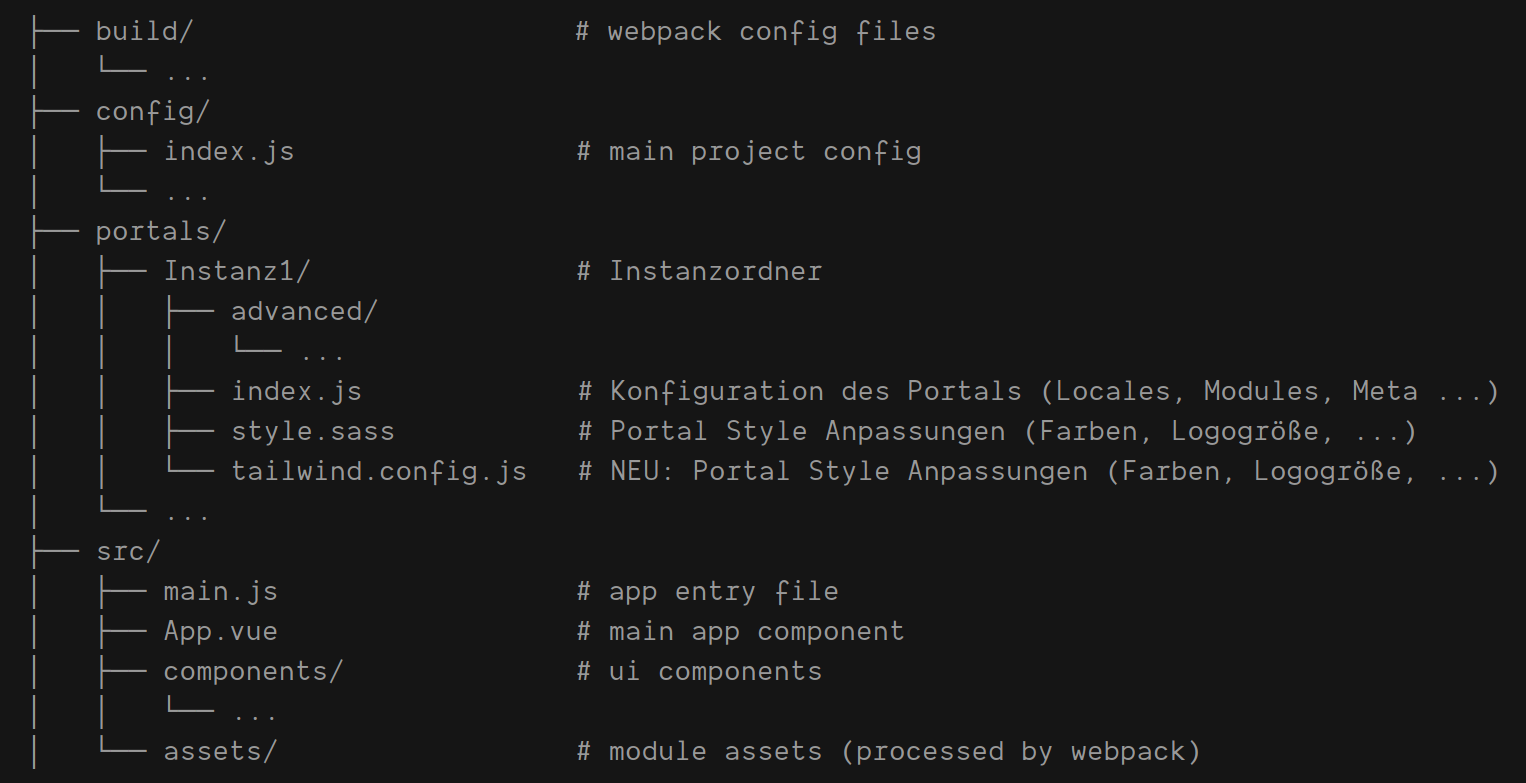
\includegraphics[width=.85\textwidth]{images/005-000-001-structureDir.png}
	\caption{Portal-Frontend Repository Struktur}
	\label{fig:structureDir}
\end{figure}

Ein Portal kann anschließend durch ein Node-Skript mit einem Portalordnernamen als Parameter transpiliert werden:

\begin{quotation}
	\emph{npm run build Instanz1}
\end{quotation}

Durch den Befehl werden die Dateien aus dem Ordner \textit{Instanz1} in die Build und Konfigurationsdateien importiert. Äquivalent könnte man eine neue Portalinstanz in dem Verzeichnis \textit{portals/Instanz2} anlegen und starten.

Da Tailwindcss standardmäßig im Root Verzeichnis nach der optionalen \textit{tailwind.config.js} sucht sind für diese Art der Instanziierung besondere Anpassungen für das Tailwind Setup im \textit{portal-frontend} notwendig.

Dazu wurde zunächst im \textit{build} Verzeichnis ein Modul anlegt, die eine normale Tailwindkonfiguration anhand des Portalnamens auflösen kann und mit der Tailwindkonfiguration aus der Komponentenbibliothek zusammenführt sowie ein erweitertes PurgeCSS Setup festlegt (vgl. Codebeispiel \ref{tailwind.js}).

\lstinputlisting[caption={Modul zur Auflösung und Zusammenführung der tailwind.config.js}, label={tailwind.js}]{code/005-000_tailwindcss/tailwind.js}

Damit dieses Modul nun für das Setup von Tailwindcss innerhalb von PostCSS angewandt wird muss die \textit{postcss.config.js} wie folgt angepasst werden.

\lstinputlisting[caption={Modul zur Auflösung und Zusammenführung der tailwind.config.js}, label={tailwind.js}]{code/005-000_tailwindcss/PostcssConf.js}

Dabei ist das Setup in Form eines Rückgabewertes einer Funktion für PostCSS nicht so häufig verbreitet. Grund dafür ist jedoch das benötigte \textit{Context (ctx)} Objekt\footnote{vgl. \url{https://github.com/postcss/postcss-load-config\#context}} was in der Webpack Konfiguration wie folgt definiert wurde:

\lstinputlisting[caption={Webpack.conf.js}, label={webpack.conf.js}]{code/005-000_tailwindcss/Webpack.conf.js}